\documentclass{beamer}

\mode<presentation> {

%\usetheme{default}
%\usetheme{AnnArbor}
%\usetheme{Antibes}
%\usetheme{Bergen}
%\usetheme{Berkeley}
%\usetheme{Berlin}
%\usetheme{Boadilla}
%\usetheme{CambridgeUS}
%\usetheme{Copenhagen}
%\usetheme{Darmstadt}
%\usetheme{Dresden}
%\usetheme{Frankfurt}
%\usetheme{Goettingen}
%\usetheme{Hannover}
%\usetheme{Ilmenau}
%\usetheme{JuanLesPins}
%\usetheme{Luebeck}
\usetheme{Madrid}
%\usetheme{Malmoe}
%\usetheme{Marburg}
%\usetheme{Montpellier}
%\usetheme{PaloAlto}
%\usetheme{Pittsburgh}
%\usetheme{Rochester}
%\usetheme{Singapore}
%\usetheme{Szeged}
%\usetheme{Warsaw}


%\usecolortheme{albatross}
%\usecolortheme{beaver}
%\usecolortheme{beetle}
%\usecolortheme{crane}
%\usecolortheme{dolphin}
%\usecolortheme{dove}
%\usecolortheme{fly}
%\usecolortheme{lily}
%\usecolortheme{orchid}
%\usecolortheme{rose}
%\usecolortheme{seagull}
%\usecolortheme{seahorse}
%\usecolortheme{whale}
%\usecolortheme{wolverine}

%\setbeamertemplate{footline} % To remove the footer line in all slides uncomment this line
%\setbeamertemplate{footline}[page number] % To replace the footer line in all slides with a simple slide count uncomment this line

%\setbeamertemplate{navigation symbols}{} % To remove the navigation symbols from the bottom of all slides uncomment this line
}

\usepackage{graphicx} % Allows including images
\usepackage{booktabs} % Allows the use of \toprule, \midrule and \bottomrule in tables
\usepackage{amsfonts}
\usepackage{mathrsfs, bbold}
\usepackage{amsmath,amssymb,graphicx}
\usepackage{mathtools} % gather
\usepackage[export]{adjustbox} % right-aligned graphics

% argmax
\DeclareMathOperator*{\argmax}{arg\,max}

%----------------------------------------------------------------------------------------
%	TITLE PAGE
%----------------------------------------------------------------------------------------

\title["13"]{13: Modal And Distributional Approximations}

% \author{Taylor} 
% \institute[UVA] 
% {
% University of Virginia \\
% \medskip
% \textit{} 
% }
\date{11/25/19} 

\begin{document}
%----------------------------------------------------------------------------------------

\begin{frame}
\titlepage 
\end{frame}


%----------------------------------------------------------------------------------------
\begin{frame}[fragile]
\frametitle{Variational Inference}

{\bf Variational inference} approximates an intractable posterior $p(\theta \mid y)$ with some chosen distribution $g(\theta \mid \phi)$ (e.g. multivariate normal).
\newline
\pause

We will assume this approximating distribution factors into $J$ components:
$$
g(\theta \mid \phi) = \prod_{j=1}^J g_j(\theta_j \mid \phi_j) = g_j(\theta_j \mid \phi_j)g_{-j}(\theta_{-j} \mid \phi_{-j}).
$$


We will find $\phi$ using an EM-like algorithm that minimizes Kullback-Leibler divergence.

\end{frame}

%----------------------------------------------------------------------------------------
\begin{frame}[fragile]
\frametitle{Variational Inference}

Kullback-Leibler divergence is ``reversed" this time:
\begin{align*}
KL(g || p) &= - \int \log \left( \frac{ p(\theta \mid y)}{g(\theta \mid \phi)} \right) g(\theta \mid \phi)\text{d}\theta  \\
&= - \int \log \left( \frac{ p(\theta, y)}{g(\theta \mid \phi)} \right) g(\theta \mid \phi)\text{d}\theta
+ \int \log p(y)g(\theta \mid \phi) \text{d}\theta \\
&= - \underbrace{\int \log \left( \frac{ p(\theta, y)}{g(\theta \mid \phi)} \right) g(\theta \mid \phi)\text{d}\theta}_{\text{variational lower bound}}
+  \log p(y) \\
\end{align*}

The term that we maximize (minimize the negative) is called the {\bf variational lower bound} aka the {\bf evidence lower bound} (ELBO).

\end{frame}

%----------------------------------------------------------------------------------------
\begin{frame}[fragile]
\frametitle{Variational Inference}

Every iteration, we cycle through all the hyper-parameters $\phi_1, \ldots, \phi_J$, and change them until convergence is reached.
\newline
\pause

Looking at $\phi_j$...
\begin{align*}
&\int \log \left( \frac{ p(\theta, y)}{g(\theta \mid \phi)} \right) g(\theta \mid \phi)\text{d}\theta \\
&=  \iint \left[\log p(\theta, y) - \log g_j(\theta_j \mid \phi_j) - \log g_{-j}(\theta_{-j} \mid \phi_{-j})\right]  \\
&\hspace{10mm} g_j(\theta_j \mid \phi_j)g_{-j}(\theta_{-j} \mid \phi_{-j})\text{d}\theta_{j}\text{d}\theta_{-j} \\
&=  \int \left[\int\log p(\theta, y)g_{-j}(\theta_{-j} \mid \phi_{-j}) \text{d}\theta_{-j}\right] g_j(\theta_j \mid \phi_j)\text{d}\theta_{j} \\
&- \int\log g_j(\theta_j \mid \phi_j)g_j(\theta_j \mid \phi_j)\text{d}\theta_j - \int \log g_{-j}(\theta_{-j} \mid \phi_{-j})g_{-j}(\theta_{-j} \mid \phi_{-j})\text{d}\theta_{-j} \\ 
&=  \int  \log \left(\frac{\tilde{p}(\theta_j)}{g_j(\theta_j \mid \phi_j)}  \right) g_j(\theta_j \mid \phi_j)\text{d}\theta_{j} + \text{constant} \tag{*}
\end{align*}

\end{frame}

%----------------------------------------------------------------------------------------
\begin{frame}[fragile]
\frametitle{Variational Inference}

We think of $\tilde{p}(\theta_j)$ as an unnormalized density 
$$
\log\tilde{p}(\theta_j) = \int\log p(\theta, y)g_{-j}(\theta_{-j} \mid \phi_{-j}) \text{d}\theta_{-j}
$$
because usually

\begin{align*}
\int \tilde{p}(\theta_j) \text{d}\theta_j &= \int \exp\left[ \int\log p(\theta, y)g_{-j}(\theta_{-j} \mid \phi_{-j}) \text{d}\theta_{-j}\right] \text{d}\theta_j \\
&\le \int \exp\left[ \log \int p(\theta, y)g_{-j}(\theta_{-j} \mid \phi_{-j}) \text{d}\theta_{-j}\right] \text{d}\theta_j \tag{Jensen's}\\
&= \iint  p(\theta, y)g_{-j}(\theta_{-j} \mid \phi_{-j}) \text{d}\theta_{-j} \text{d}\theta_j \\
&< \infty
\end{align*}

\end{frame}

%----------------------------------------------------------------------------------------
\begin{frame}[fragile]
\frametitle{Variational Inference}

\begin{block}{VI algorithm}
For $j=1,\ldots,J$ set $\phi_j$ so that $\log g_j(\theta_j \mid \phi_j)$ is equal to 
$$
\log\tilde{p}(\theta_j) = \int\log p(\theta, y)g_{-j}(\theta_{-j} \mid \phi_{-j}) \text{d}\theta_{-j}
$$
\end{block}

\end{frame}

%----------------------------------------------------------------------------------------
\begin{frame}[fragile]
\frametitle{Variational Inference: educational testing example}

When the parameters are $\alpha_1, \ldots, \alpha_8, \mu, \tau$, the log posterior is
$$
\log p(\theta \mid y) = \text{constant} - \frac{1}{2}\sum_{j=1}^8\frac{(y_j - \alpha_j)^2 }{\sigma^2_j } - 8 \log \tau - \frac{1}{2}\frac{1}{\tau^2}\sum_{j=1}^8(\alpha_j - \mu)^2
$$
and we assume
$$
g(\alpha_1, \ldots, \alpha_8, \mu, \tau) = g(\alpha_1) \times  \cdots \times g(\alpha_8) g(\mu) g(\tau).
$$

Let's reparameterize $\tau$ as $\tau^2$ and assume $g(\alpha_1), \ldots, g(\alpha_8) g(\mu)$ are all normal distributions, and $g(\tau^2)$ is an Inverse-Gamma.

  
\end{frame}


%----------------------------------------------------------------------------------------
\begin{frame}[fragile]
\frametitle{Variational Inference: example}


\begin{align*}
&\log g(\alpha_j) \\
&\overset{\text{set}}{=} \log\tilde{p}(\alpha_j) \\
&= \int\log p(\theta, y)g_{-j}(\theta_{-j}) \text{d}\theta_{-j} \\
&= - \frac{1}{2}\sum_{i=1}^8\frac{E_{-j}[(y_i - \alpha_i)^2 ] }{\sigma^2_i } - 8 E_{-j}[\log \tau] - \frac{1}{2} E_{-j}\left[\frac{1}{\tau^2}\right] \sum_{i=1}^8 E_{-j}[(\alpha_i - \mu)^2 ] + c \\
&= - \frac{1}{2}\frac{(y_j - \alpha_j)^2 }{\sigma^2_j } -  \frac{1}{2} E_{-j}\left[\frac{1}{\tau^2}\right] E_{-j}[(\alpha_j - \mu)^2 ] + c' \\
&= - \frac{1}{2}\frac{(y_j - \alpha_j)^2 }{\sigma^2_j } -  \frac{1}{2} E_{-j}\left[\frac{1}{\tau^2}\right] (\alpha_j^2 - 2\alpha_j E_{-j}[\mu] ) ] + c''
\end{align*}
We are using linearity, independence, the data aren't random, and we're grouping all the terms that don't involve $\alpha_j$ into the constant.
\newline

So $g(\alpha_j) = $...
\end{frame}

%----------------------------------------------------------------------------------------
\begin{frame}[fragile]
\frametitle{Variational Inference: example}


For $\mu$:
\begin{align*}
\log\tilde{p}(\mu) &= \int\log p(\theta, y)g_{-j}(\theta_{-j} \mid \phi_{-j}) \text{d}\theta_{-j} \\
&= - \frac{1}{2}E_{-\mu}\left[ \frac{1}{\tau^2}\sum_{j=1}^8(\alpha_j - \mu)^2\right] + \text{constant} \\
&= - \frac{1}{2}E_{-\mu}\left[ \frac{1}{\tau^2} \right] \sum_{j=1}^8 \left( \mu^2 - 2 \mu E_{-\mu}[ \alpha_j] \right) + \text{constant} \\
&= - \frac{1}{2}E_{-\mu}\left[ \frac{1}{\tau^2} \right]  \left( 8 \mu^2 - 2 \mu \sum_{j=1}^8 E_{-\mu}[ \alpha_j] \right) + \text{constant}
\end{align*}

So $g(\mu) = $...
\end{frame}

%----------------------------------------------------------------------------------------
\begin{frame}[fragile]
\frametitle{Variational Inference: example}


For $\tau$ (not $\tau^2$):
\begin{align*}
\log\tilde{p}(\tau) &= \int\log p(\theta, y)g_{-j}(\theta_{-j} \mid \phi_{-j}) \text{d}\theta_{-j} \\
&= - 8 \log \tau - \frac{1}{2}\frac{1}{\tau^2} E_{-\tau}\left[ \sum_{j=1}^8(\alpha_j - \mu)^2 \right] + c \\
\end{align*}

So $g(\tau) \propto \tau^{-8} \exp\left[-\frac{\sum_jE_{-\tau}[(\alpha_j - \mu)^2]}{2 \tau^2} \right]$ which means $$
g(\tau^2) = (\tau^2)^{-(\frac{7}{2}+1)}\exp\left[-\frac{\sum_jE_{-\tau}[(\alpha_j - \mu)^2]}{2 \tau^2} \right]
$$
which is an InverseGamma$\left( \frac{7}{2}, \frac{\sum_jE_{-\tau}[(\alpha_j - \mu)^2]}{2 }\right)$
\end{frame}

%----------------------------------------------------------------------------------------
\begin{frame}[fragile]
\frametitle{Variational Inference: example}

To complete this example, we need to derive:
\begin{itemize}
\item for $g(\alpha_j)$: 
  \begin{enumerate}
  \item $E_{-j}\left[\frac{1}{\tau^2}\right] = E_{\tau^2}\left[\frac{1}{\tau^2}\right]$, 
  \item $ E_{-j}[\mu] = E_{\mu}[\mu]$ 
  \end{enumerate}
\item for $g(\mu)$: 
  \begin{enumerate}
  \item $E_{-\mu}[ \alpha_j] = E_{\alpha_j}[ \alpha_j]$, 
  \item $E_{-j}\left[\frac{1}{\tau^2}\right] = E_{\tau^2}\left[\frac{1}{\tau^2}\right]$ 
  \end{enumerate}
\item for $g(\tau^2)$: 
  \begin{enumerate}
  \item $\sum_jE_{-\tau}[(\alpha_j - \mu)^2] = \sum_jE_{\alpha_j,\mu}[(\alpha_j - \mu)^2]$, 
  \end{enumerate}
\end{itemize}

\end{frame}

%----------------------------------------------------------------------------------------
\begin{frame}[fragile]
\frametitle{Variational Inference: example}

\begin{center}
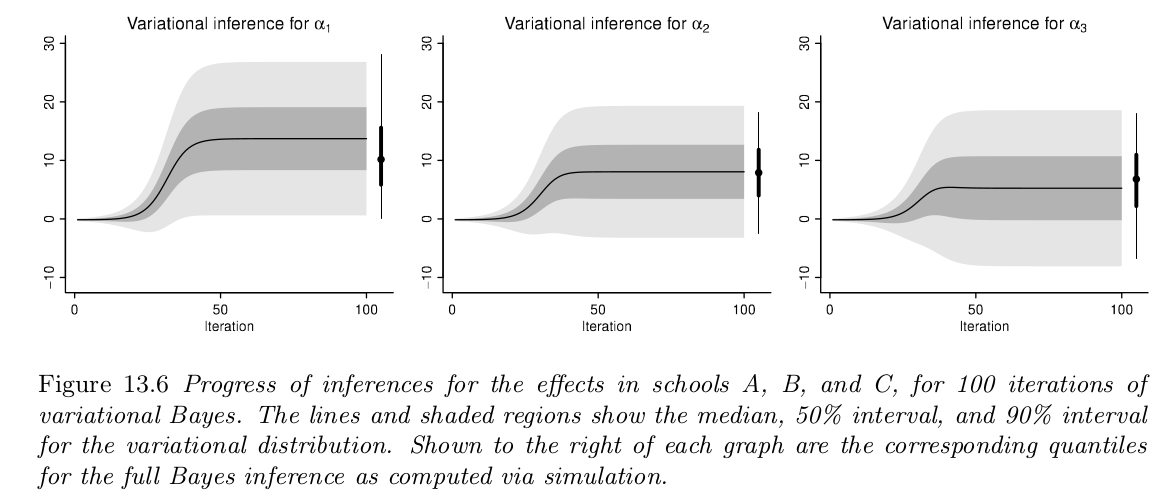
\includegraphics[width=120mm]{vi_convergence.png}
\end{center}

\end{frame}




%----------------------------------------------------------------------------------------
\begin{frame}[fragile]
\frametitle{Expectation Propagation: warmup}

$p(x \mid \theta)$ is in the exponential family if it can be written as  
$$
h(x)\exp\left[\eta(\theta)'T(x) - A(\theta) \right]
$$

Example:
$$
N(\theta \mid \mu, \sigma^2) = \frac{1}{\sqrt{2\pi\sigma^2}} \exp\left[-\frac{1}{2\sigma^2}\theta^2 + \frac{\mu}{\sigma^2}\theta - \frac{\mu^2}{2\sigma^2} \right]
$$
sufficient statistic: $(\theta^2,\theta)$

canonical/natural parameters: $(-\frac{1}{2\sigma^2}, \frac{\mu}{\sigma^2})$

\end{frame}
%----------------------------------------------------------------------------------------
\begin{frame}[fragile]
\frametitle{Expectation Propagation}

{\bf Expectation Propogation} is another deterministic iterative technique that approximates the posterior with a distribution that is in the exponential family. 
\newline

\begin{enumerate}
\item $p(\theta \mid y) = f(\theta) = \prod_{i=0}^{n} f_i(\theta)$
\item $g(\theta) = \prod_{i=0}^{n} g_i(\theta)$
\end{enumerate}

$f_0(\theta) = p(\theta)$, $f_1(\theta) = p(y_1 \mid \theta)$, ...
\newline

For more info: \url{https://arxiv.org/abs/1412.4869}
\end{frame}
%----------------------------------------------------------------------------------------
\begin{frame}[fragile]
\frametitle{Expectation Propagation}

The {\bf cavity distribution} is 
$$
g_{-i}(\theta) \propto g(\theta) / g_i(\theta),
$$
and the {\bf tilted distribution} is 
$$
g_{-i}(\theta) f_i(\theta).
$$

At each stage, we update $g_i(\theta)$ so that we ``target" $g_{-i}(\theta) f_i(\theta)$ with $g(\theta)$. 


\end{frame}

%----------------------------------------------------------------------------------------
\begin{frame}[fragile]
\frametitle{Expectation Propagation}

At each stage, we update $g_i(\theta)$ so that we ``target" $g_{-i}(\theta) f_i(\theta)$ with $g(\theta)$. 
\newline

Notice that
$$
\frac{\text{target}}{\text{``proposal"} } = \frac{g_{-i}(\theta) f_i(\theta)}{g(\theta)} = \frac{f_i(\theta)}{g_i(\theta)}.
$$

However, we cannot ignore the cavity distribution in each ``site" update. This is because we choose $g(\theta)$ so that its {\bf moments match} those of $g_{-i}(\theta) f_i(\theta)$. This is like choosing $g_i(\theta)$ to approximate $f_i(\theta)$ {\bf in the context of} $g_{-i}(\theta)$.

\end{frame}

%----------------------------------------------------------------------------------------
\begin{frame}[fragile]
\frametitle{Expectation Propagation}

If $g(\theta) = \text{Normal}(\mu, \Sigma)$, for each $i$ we change $\mu$ and $\Sigma$ by solving
$$
\mu \overset{\text{set}}{=} E_{\text{tilted }i}[\theta] 
$$
and
$$
\Sigma \overset{\text{set}}{=} \operatorname{Var}_{\text{tilted }i}[\theta] 
$$
where $E_{\text{tilted }i}[\theta] = \int \theta g_{-i}(\theta)f_i(\theta) \text{d}\theta $ and $\operatorname{Var}_{\text{tilted }i}[\theta] = \int (\theta-\mu)(\theta-\mu)' g_{-i}(\theta)f_i(\theta) \text{d}\theta $.
\newline

The hard part is integrating.
\end{frame}
%----------------------------------------------------------------------------------------
\begin{frame}[fragile]
\frametitle{Expectation Propagation: example}

Let $\theta$ be a vector of regression parameters for a logistic regression:
\begin{align*}
p(\theta \mid y) &\propto \prod_{i=1}^n p(y_i \mid \theta)p(\theta) \\
&= \prod_{i=0}^n f_i(\theta) \\
&= f_0(\theta) \prod_{i=1}^n [\text{invlogit}(X_i'\theta )]^{y_i}[1-\text{invlogit}(X_i'\theta)]^{m_i - y_i}
\end{align*}

and choose $g(\theta)$ to be $\text{Normal}(\mu, \Sigma)$

\end{frame}
%----------------------------------------------------------------------------------------
\begin{frame}[fragile]
\frametitle{Expectation Propagation: example}

We choose $g(\theta)$ to be $\text{Normal}(\mu, \Sigma)$:
\begin{align*}
g(\theta) 
&\propto \prod_{i=0}^n \exp\left[-\frac{1}{2}(\theta - \mu_i)'\Sigma^{-1}_i(\theta - \mu_i)  \right] \\
&\propto  \exp\left[-\frac{1}{2}\sum_{i=0}^n\left( \theta'\Sigma^{-1}_i\theta - 2 \mu_i' \Sigma^{-1}_i\theta \right) \right] \\
&=  \exp\left[-\frac{1}{2}\left( \theta'\left[\underbrace{ \sum_{i=0}^n \Sigma^{-1}_i}_{\Sigma^{-1} }\right] \theta - 2 \left[\underbrace{\sum_{i=0}^n\mu_i' \Sigma^{-1}_i}_{ \text{natural param 2} } \right]\theta \right) \right]
\end{align*}

Algorithmically, $\mu, \Sigma$ change at each iteration.
\end{frame}

%----------------------------------------------------------------------------------------
\begin{frame}[fragile]
\frametitle{Expectation Propagation: example}


$g(\theta)$ is $\text{Normal}(\mu, \Sigma)$:
\begin{align*}
g(\theta) 
&\propto   \exp\left[-\frac{1}{2}\left( \theta'\left[\underbrace{ \sum_{i=0}^n \Sigma^{-1}_i}_{\Sigma^{-1} }\right] \theta - 2 \left[\underbrace{\sum_{i=0}^n\mu_i' \Sigma^{-1}_i}_{ \Sigma^{-1}\mu } \right]\theta \right) \right]
\end{align*}

Step 1: determine cavity distribution. $g_{-i}(\theta) = \text{Normal}(\mu_{-i}, \Sigma_{-i})$ where
$$
\Sigma_{-i}^{-1} = \Sigma^{-1} - \Sigma_{i}^{-1}
$$
and
$$
\Sigma_{-i}^{-1}\mu_{-i} = \Sigma^{-1}\mu - \Sigma_{i}^{-1}\mu_{i}
$$
\end{frame}

%----------------------------------------------------------------------------------------
\begin{frame}[fragile]
\frametitle{Expectation Propagation: example}


Step 2: find cavity distribution for $\eta = X_i'\theta$. 
\newline

Because any linear transformation of normals is normal and because $g_{-i}(\theta) = \text{Normal}(\mu_{-i}, \Sigma_{-i})$:
$$
g_{-i}(\eta) = \text{Normal}(M_{-i}, V_{-i}) 
$$
where 
$M_{-i} = X_i'\mu_{-i}$ and $V_{-i} = X_i'\Sigma_{-i}X_i$.

\end{frame}

%----------------------------------------------------------------------------------------
\begin{frame}[fragile]
\frametitle{Expectation Propagation: example}


Step 3: define the unnormalized tilted distribution
$$
g_{-i}(\eta)f_i(\eta) = g_{-i}(\eta)\text{Binomial}(m_i, \text{invlogit}(\eta)).
$$
and find its expectations numerically with the Gauss-Kronrod quadrature method:
\begin{align*}
E_k &= \int_{-\infty}^{\infty} \eta^k g_{-i}(\eta)f_i(\eta) \text{d}\eta \\
&\approx \int_{M_{-i}- \delta \sqrt{V_{-i}} }^{M_{-i}+ \delta \sqrt{V_{-i}}} \eta^k g_{-i}(\eta)f_i(\eta) \text{d}\eta \\
\end{align*}
for $k=0,1,2$ and $\delta$ is some large number (e.g. $10$). Finally compute $M = E_1/E_0$ and $V = E_2/E_0 - (E_1/E_0)^2$ and set $g(\eta) = \text{Normal}(M,V)$.

\end{frame}

%----------------------------------------------------------------------------------------
\begin{frame}[fragile]
\frametitle{Expectation Propagation: example}

In the previous steps we found $g(\eta) = \text{Normal}(M,V)$ and $g_{-i}(\eta) = \text{Normal}(M_{-i}, V_{-i}) $.
\newline


Step 4: find $g_i(\eta) = \text{Normal}(M_i, V_i)$:
\begin{align*}
g_i(\eta) &= g(\eta)/g_{-i}(\eta)  \\
&\propto \frac{ \exp\left[-\frac{1}{2V}\eta^2 + \frac{M}{V}\eta  \right] }{\exp\left[-\frac{1}{2V_{-i} }\eta^2 + \frac{M_{-i} }{V_{-i} }\eta  \right] } \\
&= \exp\left[-\frac{1}{2} \left(\underbrace{ \frac{1}{V} - \frac{1}{V_{-i} }  }_{\frac{1}{V_i}} \right)\eta^2 + \left( \underbrace{\frac{M}{V} - \frac{M_{-i} }{V_{-i} }}_{\frac{M_i}{V_i} } \right) \eta  \right] 
\end{align*}

\end{frame}

%----------------------------------------------------------------------------------------
\begin{frame}[fragile]
\frametitle{Expectation Propagation: example}


Step 5: find $g_i(\theta)$.
\newline

$$
g_i(\theta) = \text{Normal}(\mu_i, \Sigma_i)
$$
where 
$$
\Sigma_i^{-1} \mu_i = X_i \frac{M_i}{V_i} 
$$
and
$$
\Sigma_i^{-1} = X_i \frac{1}{V_i}X_i'
$$

\end{frame}

%----------------------------------------------------------------------------------------
\begin{frame}[fragile]
\frametitle{Expectation Propagation: example}


Step 6: find $g(\theta) \propto g_i(\theta)g_{-i}(\theta)$.
\newline

\begin{align*}
g(\theta) 
&\propto   \exp\left[-\frac{1}{2}\left( \theta'\left[\underbrace{ \sum_{i=0}^n \Sigma^{-1}_i}_{\Sigma^{-1} }\right] \theta - 2 \left[\underbrace{\sum_{i=0}^n\mu_i' \Sigma^{-1}_i}_{ \Sigma^{-1}\mu } \right]\theta \right) \right]
\end{align*}

$$
\Sigma^{-1}\mu = \overbrace{\Sigma^{-1}_{-i}\mu_{-i}}^{\text{from step 1} } + \overbrace{\Sigma^{-1}_{i}\mu_{i}}^{\text{from step 5}}
$$
and
$$
\Sigma^{-1} = \underbrace{\Sigma^{-1}_{-i}}_{\text{from step 1} } + \underbrace{\Sigma^{-1}_i}_{\text{from step 5}}
$$

\end{frame}


% ----------------------------------------------------------------------------------------
\begin{frame}
  \frametitle{Discussions of Variational Bayes and Expectation Propagation}
  \begin{itemize}
  \item EM algorithm for finding posterior mode of $p(\phi \mid y)$ can be thought of as a special case of variational Bayes by treating (a) $g(\phi)$ is a point mass (b) $g(\gamma)$ is of the form $g(\gamma \mid \phi, y)$ but unconstrained to any family of distribution.
  \item Moment matching of EP corresponds to minimizing the Kullback-Leibler divergence from the tilted distribution and to the new approximated distribution $g(\theta)$. But no guarantee that the KL divergence between the posterior distribution and the approximated distribution is decreasing.
  \end{itemize}
\end{frame}


% ----------------------------------------------------------------------------------------
\begin{frame}
  \frametitle{Discussions of Variational Bayes and Expectation Propagation}
  \begin{itemize}
  \item Both VI and EP have more generalized form by revising the KL divergence.
  \item Both VI and EP can serve as the proposal distribution and be incorporated into importance sampling/resampling framework.
  \end{itemize}
  \end{frame}
\end{document} 
